% Fair topics for CS340 MIDTERM:
% \begin{enumerate}
%     \item test vs. training
%     \item decision trees
%     \item decision stumps
%     \item naive Bayes
%     \item k-nn
%     \item ensemble methods
%     \item clustering
%     \item outlier detection
%     \item least squares
%     \item norms
%     \item change of bases (polynomial bases)
%     \item log-sum-exp
%     \item huber
%     \item gradient descent
%     \item linear 
%     \item nearest neighbors
%     \item k-means clustering
%     \item naive Bayes
%     \item Probabilistic classification
%     \item cross validation
% \end{enumerate}

\documentclass{article}

\usepackage{fullpage}
\usepackage{color}
\usepackage{amsmath}
\usepackage{url}
\usepackage{verbatim}
\usepackage{graphicx}
\usepackage{parskip}
\usepackage{amssymb}
\usepackage{amsfonts}
\usepackage{nicefrac}
\usepackage{listings} % For displaying code
\usepackage{algorithm2e} % pseudo-code
\usepackage{natbib}
\usepackage{todonotes}
\usepackage{caption}
\usepackage{subcaption}
% Answers
\def\rubric#1{\gre{Rubric: \{#1\}}}{}
\def\ans#1{\par\gre{Answer: #1}}
% Colors
\definecolor{blu}{rgb}{0,0,1}
\def\blu#1{{\color{blu}#1}}
\definecolor{gre}{rgb}{0,.5,0}
\def\gre#1{{\color{gre}#1}}
\definecolor{red}{rgb}{1,0,0}
\def\red#1{{\color{red}#1}}
\def\norm#1{\|#1\|}
\usepackage{xcolor}
\usepackage{listings}


\definecolor{codegreen}{rgb}{0,0.6,0}
\definecolor{codegray}{rgb}{0.5,0.5,0.5}
\definecolor{codepurple}{rgb}{0.58,0,0.82}
\definecolor{backcolour}{rgb}{0.95,0.95,0.92}

\lstdefinestyle{mystyle}{
    backgroundcolor=\color{backcolour},   
    commentstyle=\color{codegreen},
    keywordstyle=\color{magenta},
    numberstyle=\tiny\color{codegray},
    stringstyle=\color{codepurple},
    basicstyle=\ttfamily\footnotesize,
    breakatwhitespace=false,         
    breaklines=true,                 
    captionpos=b,                    
    keepspaces=true,                 
    numbers=left,                    
    numbersep=5pt,                  
    showspaces=false,                
    showstringspaces=false,
    showtabs=false,                  
    tabsize=2
}

\lstset{style=mystyle}
% Math
\def\R{\mathbb{R}}
\def\argmax{\mathop{\rm arg\,max}}
\def\argmin{\mathop{\rm arg\,min}}
\newcommand{\mat}[1]{\begin{bmatrix}#1\end{bmatrix}}
\newcommand{\alignStar}[1]{\begin{align*}#1\end{align*}}
\def\half{\frac 1 2}

% LaTeX
\newcommand{\fig}[2]{\includegraphics[width=#1\textwidth]{#2}}
\newcommand{\centerfig}[2]{\begin{center}\includegraphics[width=#1\textwidth]{#2}\end{center}}
\def\items#1{\begin{itemize}#1\end{itemize}}
\def\enum#1{\begin{enumerate}#1\end{enumerate}}

\begin{document}

\title{CPSC 340 Machine Learning Take-Home Midterm Exam\\ (Fall 2020)}


\section*{Question 2}
\setcounter{section}{0}

\section{Team}
\begin{tabular}{|c | c | c |} 
\hline
Team Members & \emph{Shuyang Ye} & \emph{Jinlin Zhu} \\
\hline
Student ID & \emph{96481163} & \emph{96057468} \\
\hline
CS ID & \emph{l8n8s} & \emph{q6j8i} \\
\hline
\end{tabular}
\begin{tabular}{|c | c |} 
\hline
Kaggle Team Name & \emph{TESNO.1}\\
\hline
\end{tabular}
\section{Solution Summary}
    Three different methods are adopted individually. The most intuitive and simplest model is to use only Canada's past deaths to predict future deaths. The predicted future deaths curve is a straight line which means the daily deaths is a constant. The second method calculates the daily deaths and adopts Auto Regression model to predict the future daily deaths and then the future total deaths. In the end, I stack this two method together to predict the final result.
    
    Third method is to consider the impact from other countries. Given that case density is more informative than the total number of cases for national outbreak correlation analysis, we used the total national death toll density as an indicator to calculate the \textbf{Cross Correlation} between different countries, thus selecting countries with similar outbreaks. Thus we can establish a linear map between deaths density of other countries and Canada. Using AR model own each other countries to predict the future deaths, then using the linear map to predict the deaths of Canada.
    
    Finally we adopted the third method that is to combine factors of impact from other countries and the spec country "Canada" together.
    
\section{Experiments}
The formula we used to predict the future deaths of Canada is  Deaths(CA,Future) = Num\_people\_100k * Deaths\_100k(CA,Future) and 
\subsection{Auto Regression Model}
As for the final method, we used this model to predict the short term future of feature "deaths\_100k" of all countries. We coded two classes called My\_AutoReg and AutoReg1 in "AutoRegression.py" file based on the same algorithm provided by instructions of the Question 2. 
\subsection{Select lags}
The main hyper-parameter of AR model is the lags we used to generate the Matrix X, by which we predict the value of next day based on the past "num=lags" days. We choose lags by plotting the Partial Autocorrelation Plot (Figure (a)), we can see that only first two past days have significant impact on the value of the present day. Thus we choose \textbf{Lags = 2}. We adopted the same lags for all countires future predicitons.

\subsection{Multivariable Linear Regression Model}
We adopted Linear Regression for feature "deaths\_100k" of all NearestNeighbors Countries as X and the feature "deaths\_100k" of Canada as y. Thus we could get a Linear relationship and could make "Parallel" Predictions to the death density of Canada.

\subsection{Select N Nearest Neighbors}
We finally used the \textbf{Cross Correlation} to measure "distances" between other countries. This distances is actually the similarities. We noticed that the deaths density between two selected countries have significantly higher correlation. However, the starting date of the pandemic outbreak of each country is different by days. So we created a loop to shift the deaths\_100k data from other countries by "num=lag\_country" days until they has their best correlation with the spec country "CA". \\
We used these nearest countries to implement a multivariable linear regression from their feature "deaths\_100k" as Input Matrix X to the feature "deaths\_100k" of the spec country "CA" as y vector. We selected the period of 269 days as training set and newest 11 days as validation set. We ploted training error plots vs N\_Nearest\_Neighbors as Figure (b). For training phase, we adopted "elbow" method and find approximate best num is 7 or 8 or 9. We chose \textbf{N\_Nearest\_Neighbors = 7} in the end.
 
\begin{figure}
\centering
\begin{subfigure}{.5\textwidth}
  \centering
  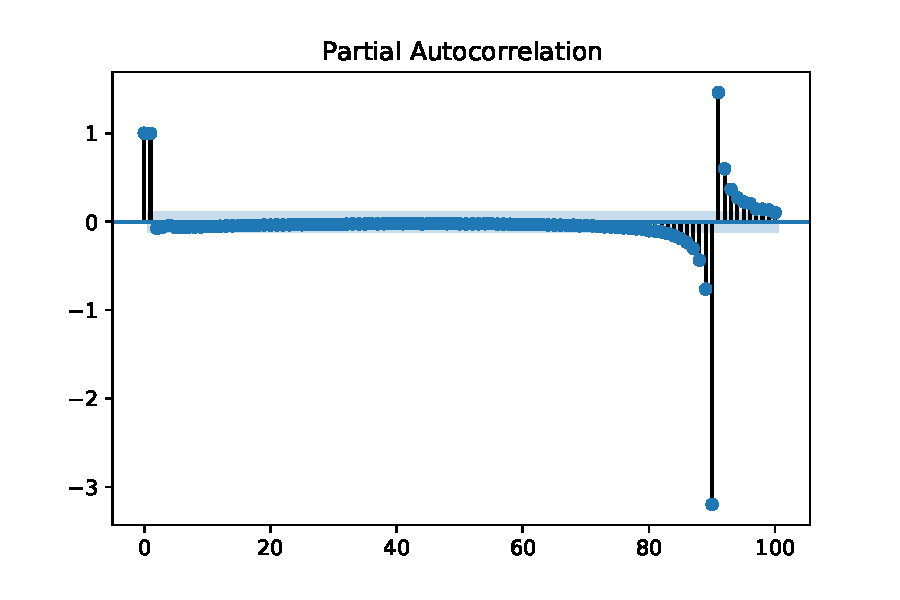
\includegraphics[width=.9\linewidth]{figs/pacf_lag_plot_CA.pdf}
  \caption{PACF plot of feature "deaths\_100k" of Canada}
  \label{fig:sub1}
\end{subfigure}%
\begin{subfigure}{.5\textwidth}
  \centering
  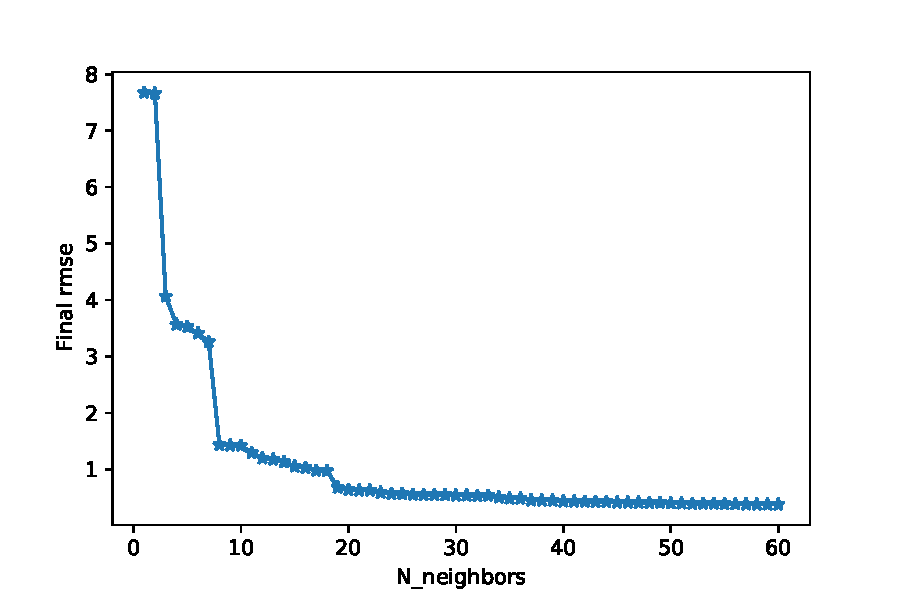
\includegraphics[width=.9\linewidth]{figs/Find_N_plot_d11_CA_train.pdf}
  \caption{Training Error vs N\_Nearest\_Neighbors plot }
  \label{fig:sub2}
\end{subfigure}
\label{fig:test}
\end{figure}
\section{Results}

\begin{center}
 \begin{tabular}{|c | c | c |} 
 \hline
 Team Name & Kaggle Phase 1 Score & Kaggle Phase 2 Score  \\ [0.5ex]
 \hline\hline
 \emph{TESNO.1} & \emph{10.865}  & \emph{459.16159}  \\
 \hline
\end{tabular}
\end{center}

\section{Conclusion}
The final result is good enough according to our very simple model. We have learned how to code the Auto Regression model, how to select features and hyper-parameters of our models in practice. We could try more features and created more sophisticated modesl if given more time.
\newpage
\section{Code}
\lstinputlisting[language=python]{main.py}
\lstinputlisting[language=python]{AutoRegression.py}
\lstinputlisting[language=python]{country.py}
\lstinputlisting[language=python]{utils.py}
\lstinputlisting[language=python]{linear_model.py}
\lstinputlisting[language=python]{findMin.py}


\end{document}
